\subsection{Evaluation}
Dans cette section, nous présentons une évaluation approfondie de notre implémentation sur une grande variété de charges de travail.
Nous commençons par lister les différentes métriques pour tester la performance de notre contribution, par la suite nous allons décrire notre configuration de test, puis nous explorons en détail la migration de plusieurs charges de travail en détail.
Notez qu'aucune des expériences de cette section n'utilise les options d'optimisation citée en annexe, car nous avons souhaité mesurer les performances de base de notre système.


\subsubsection{Métrique de performances}
Une bonne stratégie de migration ne cherche pas seulement à déplacer une VM d'un endroit à un autre aussi rapidement que possible, mais doit aussi minimiser ses effets secondaires.
On peut mesurer l'efficacité d'un algorithme de migration grâce à ces métriques :

\begin{description}
\item[Temps total de migration]
Il s'agit de la durée entre le moment où la migration est initiée et le moment où la VM migrée est reprise sur le serveur de destination et qu'il ne reste aucune donnée à transférer depuis le site source.
\item[Temps d'arrêt (Downtime)] Il s'agit de la durée pendant laquelle la VM migrée est hors service.
Cette mesure détermine le degré de transparence de la migration pour les utilisateurs de la VM migrée.
Pour une migration non live, le temps total de migration est égal au temps d'arrêt.
\item[Trafic réseau total]
Cette mesure représente le total des données transférées pendant la migration.
Il s'agit d'une mesure critique lorsque la machine virtuelle migrée exécute un service à forte intensité de réseau, car elle se disputera la bande passante du réseau avec le processus de migration.
\end{description}

Les seules métriques nous permettant d'analyser les performances de notre solution sont le temps total et le temps d'arrêt.
En effet, le trafic réseau total n'est pas prise en compte pour analyser les performances de notre implémentation, car notre modification ne transfère aucune donnée sur le flux de la migration.


\subsubsection{Machine de test}
Nous effectuons des migrations de test sur une machine en local pour mieux observer l'impact de notre algorithme de hash avec comme bottleneck notre processeur.
La machine est équipée d'un processeur Intel® Core™ i7-1065G7 (8MB Cache, jusqu'a 3.9 GHz), d'une ram de 16GO avec une fréquence de 4267Mhz.

\subsubsection{Impact des charges de travail sur la migration}


Afin d'étudier un seul facteur, nous avons fixé des valeurs pour tous les paramètres, à l'exception des paramètres étudiés, et nous avons mesuré à la fois le temps d'arrêt et le temps total de migration à différents niveaux du paramètre étudié.

\begin{description}
\item[VM size]

Nous avons étudié le temps de migration des VM inactives avec VMSIZE configuré à 512 Mo, 1 Go, 2 Go, 4 Go et 8 Go de RAM.
Les machines virtuelles étaient inactives, aucun processus générateur de charge n'a été utilisé.

\begin{figure}[H]
\begin{minipage}{0.48\textwidth}
\centering
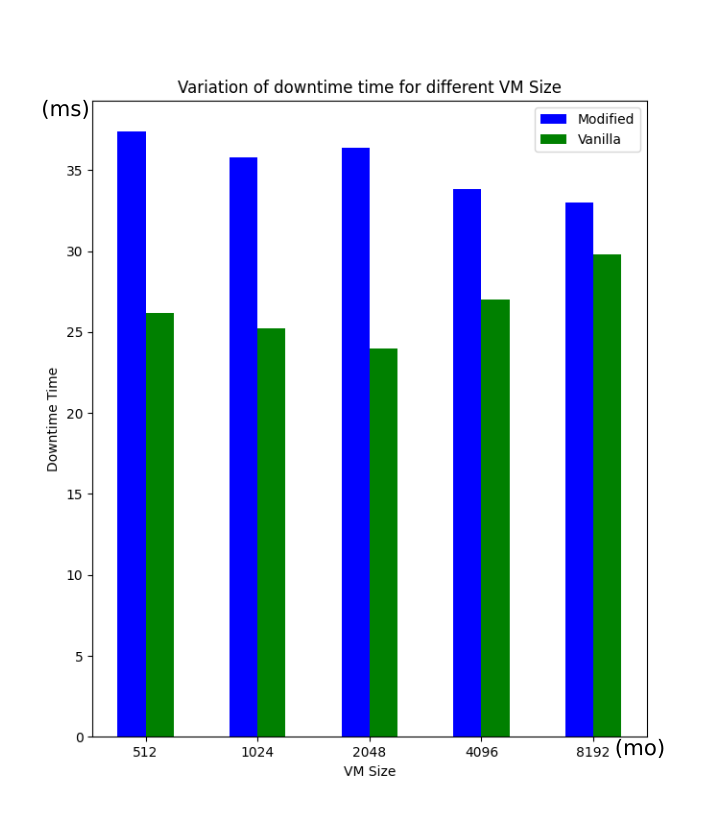
\includegraphics[width=1\linewidth]{include/down_vmsize.png}
\end{minipage}\hfill
\begin{minipage}{0.48\textwidth}
\centering
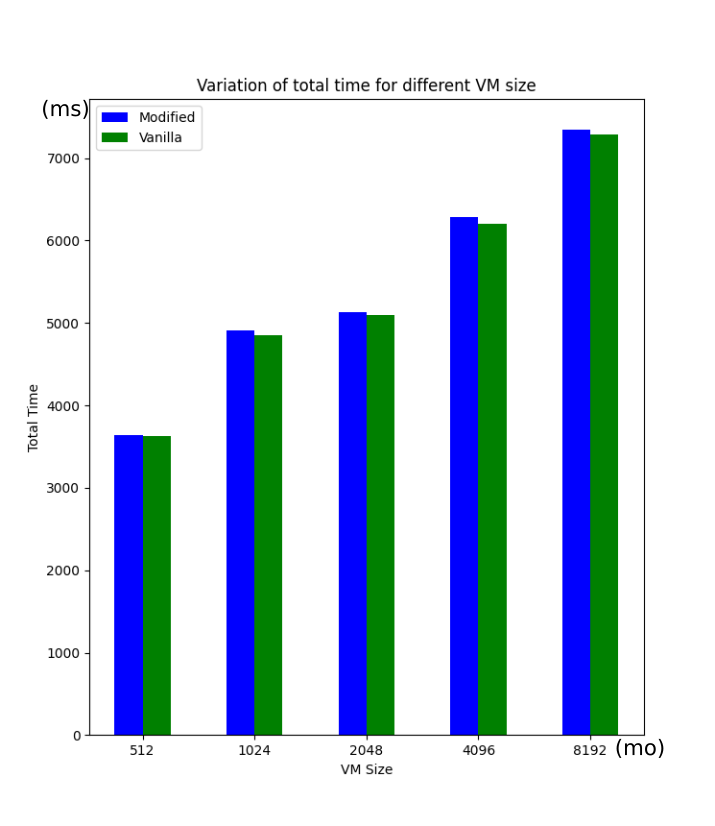
\includegraphics[width=1\linewidth]{include/total_vmsize.png}
\end{minipage}
\caption{Différence de downtime et du temps total pour la version par défaut et la version modifiée}
\end{figure}

\item[Dirty rate]
Afin de s'appuyer sur les mécanismes de trappe et de table des pages du système d'exploitation, toutes les approches de migration de VM copient le contenu de la mémoire en pages.
Par conséquent, une page entière doit être migrée même si seulement une fraction de la page est écrite.
Nous avons testé cette hypothèse en modifiant quelques octets en utilisant un script générant des pages sales au sein de la machine virtuelle.
Ce programme prend en paramètre la vitesse de génération de nouvelles pages sales (Dirty rate).

Nous avons remarqué que si l'on dépasse un dirty rate de 30\% la migration dans les deux cas (avec et sans modification) n'arrive pas à converger.
Pour nos résultats nous avons pris des vitesses de 0\%, 10\% et 20\%.

\begin{figure}[H]
\begin{minipage}{0.48\textwidth}
\centering
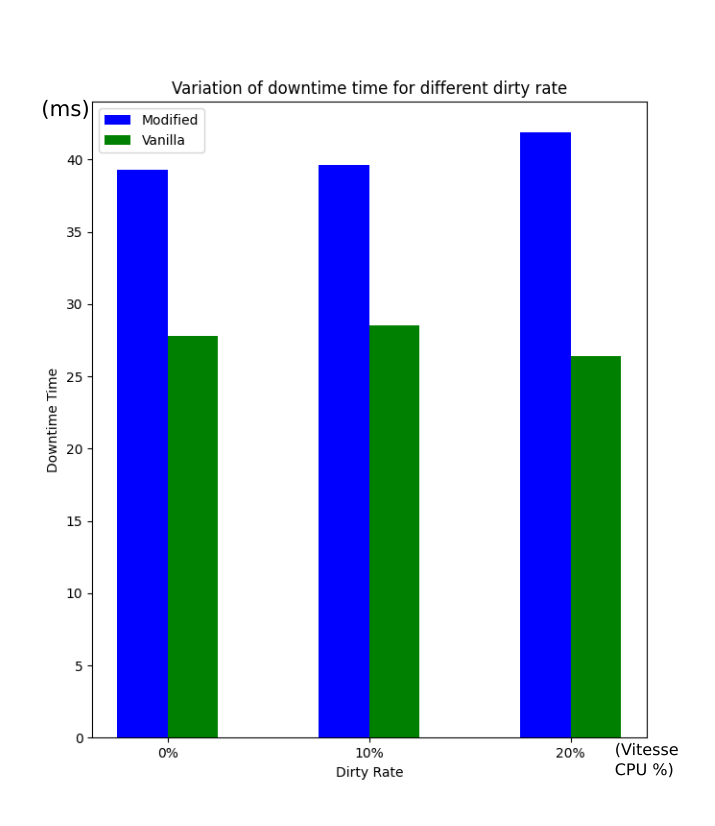
\includegraphics[width=1\linewidth]{include/down_rate.png}
\end{minipage}\hfill
\begin{minipage}{0.48\textwidth}
\centering
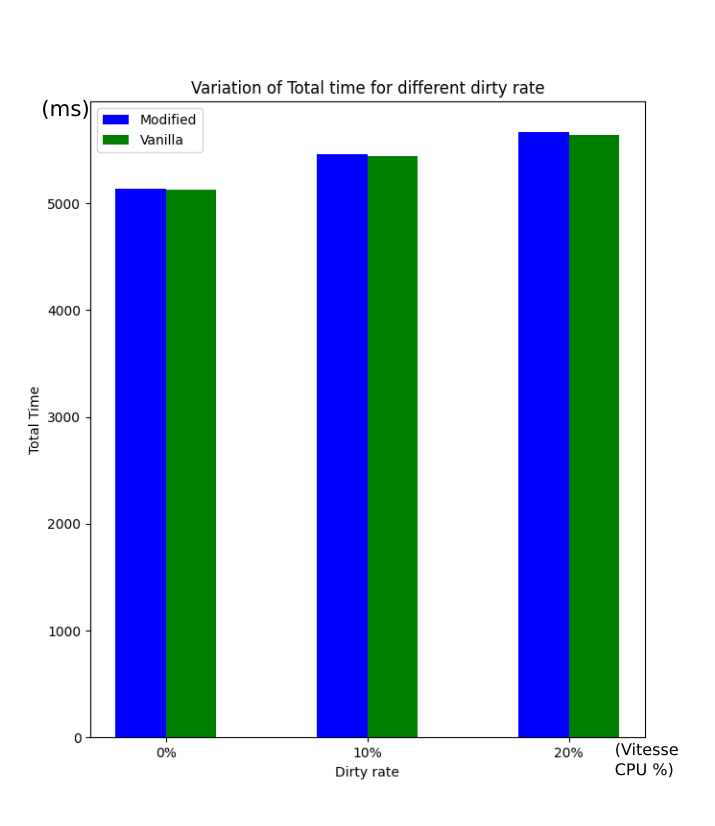
\includegraphics[width=1\linewidth]{include/total_rate.png}
\end{minipage}
\caption{Différence de downtime et du temps total pour la version par défaut et la version modifiée}
\end{figure}


\end{description}

En comparant les figures, nous pouvons constater que le temps d'arrêt présente un comportement très différent de celui du temps de migration, bien que le premier fasse partie du second.
Cela n'est pas surprenant, car une utilisation accrue de la mémoire (plus de pages écrites à un rythme croissant) nécessite le transfert de plus de mémoire dans la phase d'arrêt et de copie.

Notre implémentation rajoute un overhead d'en moyenne de 10 ms, c'est une valeur plus qu'acceptable, car la limite décrite dans QEMU pour passer à la phase 3 est de 300 ms.

En terme de pourcentage, pour l'overhead en phase de downtime nous obtenons une valeur de 40\% en plus.
Ceci est principalement lié au calcul de hash finale qui doit être faite dans la phase de downtime.
Cela parait énorme, mais il faudrait un overhead de 10000\% pour atteindre les 300 ms limite.
Cependant, l'overhead en temps total est de l'ordre de moins de 1\%, cela veut dire que le temps de calcul de l'empreinte est presque inclus dans le temps de transfert du flux.
Il faut prendre aussi en compte que le transfert est fait en local avec donc le CPU comme bottleneck.
\subsubsection{Proposition d'optimisation}

\begin{description}
    \item[Calcul du hash dans un thread différent] Dans notre implémentation, la génération de l'empreinte de la machine virtuelle se fait sur le même fil d'exécution que l'envoi des données sur le réseau.
    Dans un système où le réseau est le bottleneck, l'overhead induit par le hachage des données et de leur envoi est négligeable par rapport au temps de transfert.    
    Nous pouvons gagner quelques millisecondes en ayant deux threads parallèles lors de la génération de l'empreinte de la machine virtuelle: l'un va calculer le hash des données et l'autre va transférer les données sur le réseau.
    \item[Hashage intelligent des pages dirty] Cette optimisation consiste à créer un cache avec un algorithme d'éviction LRU.
    Le but ici est de ne pas hasher les données qui sont constamment modifiées mais à la place d'inclure dans le calcul de l'empreinte seulement les pages/blocs qui n'ont pas été modifiées depuis un certain temps.
    L'optimisation se découpe en plusieurs points :
    \begin{itemize}
    \item En tête de liste nous aurons les pages qui ont été modifiées le plus récemment, qui ont donc une grande probabilité à être modifié à nouveau.
    \item En queue de liste nous aurons les pages qui sont les plus anciennement modifiées, et donc ont moins de chance d'être modifiées.
    \item Si une page est évincée de la liste alors son contenu sera hashé.
    \item À la dernière phase de la migration (la phase d'arrêt de la machine source) la liste pourra être parcouru et le contenu des pages dirty restantes sera hashé. 
    La machine source étant arrêtée, il est impossible que les données changent.
    \end{itemize}
    \item[Hashage intelligent des pages vides] Cette optimisation consiste à éviter de hasher les pages/blocs qui sont initialisés avec des zéros ainsi que les pages non utilisées.
    \item[Hashage des données plus fin] Cette optimisation consiste à éviter d'inclure le header des sections dans le calcul de l'empreinte de la machine virtuelle.
\end{description}
    Toutes ces optimisations ont pour but de réduire la quantité des données incluse dans la génération de l'empreinte de la machine virtuelle et ainsi réduire la pression sur le CPU. 
    Ces optimisations ont permis de réduire l'overhead de notre implémentation.
    